\chapter{Phase III: Implementierung}

Nach der ersten Iteration der Design-Phase war die grunds�tzliche Architektur und Funktionsweise des \DevEnvs\ festgelegt. In der Implementierungs-Phase wurde das Design in \C++/CLI und \Csharp\ mit Visual Studio 2008 Service Pack 1 umgesetzt. Es wurde eine Vielzahl an \emph{Third Party} Bibliotheken und Frameworks eingesetzt, um den Programmierungsaufwand m�glichst gering zu halten.

Zun�chst wurde mit der Umsetzung des DLL-\emph{Replacement}-Mechanismus begonnen, dann wurde das GUI-Framework implementiert. Anschlie�end wurden die einzelnen Systemanforderungen inkrementell programmiert. Durch das inkrementelle Vorgehen konnten schnell die ersten Features umgesetzt und getestet und dadurch auch fr�h m�gliche Designfehler entdeckt werden. Die Einf�hrung der \emph{Callbacks} wurde beispielsweise w�hrend der Umsetzung des Szenengraph-Explorers vorgenommen, bevor die erste Zeile f�r die Ressourcen oder die Profiling-Daten geschrieben worden war.

Da die wichtigsten Entscheidungen bereits w�hrend der Analyse- und Design-Phasen getroffen worden waren, konnte das Design z�gig umgesetzt werden. In den folgenden Abschnitten werden nun wichtige technische Details erl�utert, die in den vorherigen Phasen noch keine Rolle spielten. Dabei wird allerdings weitestgehend auf das Abdrucken von Code verzichtet und nur die verwendeten Konzepte erl�utert. Der komplette Source Code befindet sich auf der beiliegenden CD-ROM.

\section{Verwendete Technologien und Frameworks}
Zur Umsetzung des \DevEnvs\ wurde auf kommerzielle und frei verf�gbare Open Source Bibliotheken und Frameworks zur�ckgegriffen, um gewisse Standardl�sungen nicht selbst entwickeln zu m�ssen. Insbesondere basiert das System auf dem .NET Framework von Microsoft\footnote{\url{http://www.microsoft.com/NET}}.

\subsection{.NET Framework}
2002 ver�ffentliche Microsoft das .NET Framework, welches seither stark erweitert und verbessert wurde. �hnlich wie bei Java wird der Code zun�chst in eine Zwischensprache, die \emph{Common Intermediate Language}, �bersetzt und dann zur Laufzeit von der \emph{Common Language Runtime} (CLR) mit einem \emph{Just-in-Time-Compiler} in Maschineninstruktionen umgewandelt. Das .NET Framework spezifiziert ein vereinheitlichtes Typsystem, das \emph{Common Type System}, bietet die M�glichkeit f�r \emph{Reflection} und Code Generierung zur Laufzeit und verwendet einen \emph{Garbage Collector} zum Aufr�umen und Verwalten des Speichers. Inzwischen gibt es viele Sprachen, die in die \emph{Common Intermediate Language} �bersetzt werden k�nnen und somit Zugriff auf alle Klassen des .NET Frameworks besitzen. Die wichtigsten sind \Csharp, Visual Basic .NET und \C++/CLI \cite{dotnet}. 

Das Framework und \Csharp\ sind ECMA- und ISO-standardisiert. Es gibt verschiedene Implementierungen des Frameworks, wobei Microsoft offiziell nur Windows, mobile Ger�te wie Handys oder Zune und die XBOX 360 unterst�tzt. F�r Linux- und Mac-Systeme ist Mono\footnote{\url{http://www.mono-project.com/Main_Page}} weit verbreitet.

Das \DevEnv\ ist in \Csharp\ 3.0 und \C++/CLI implementiert. Es ist jedoch nur unter Windows lauff�hig, da sowohl der Client als auch der Server native, Windows-spezifische Funktionen und Bibliotheken verwenden. Dieser Nachteil wurde jedoch bewusst in Kauf genommen, da die Verwendung des .NET Frameworks und der plattform-abh�ngigen Bibliotheken eine einfachere und schnellere Implementierung erm�glichte.

Neben der \emph{Base Class Library}, die nur grundlegende Klassen wie Ein-/Ausgabestreams, Dateizugriffe, Strings, Listen, Hash-Tabellen und Warteschlangen anbietet, verwendet das \DevEnv\ vor allem auch Windows Forms (WinForms) f�r die Umsetzung der GUI, die Windows Communication Foundation (WCF) f�r die Interprozesskommunikation und Language Integrated Queries (Linq) f�r Filterung und Sortierung von Listen. Windows Forms basiert auf der mit Windows 95 eingef�hrten Win32-API und wurde mit dem Update auf .NET 3.0 durch die modernere Windows Presentation Foundation (WPF) abgel�st. Dennoch wird Windows Forms aufgrund seiner Einfachheit und hohen Effizienz -- sowohl bei der Entwicklung als auch beim Laufzeitverhalten -- gerne noch f�r Anwendungen eingesetzt, die keine speziellen Anforderungen, wie \emph{Themes} oder Animationen, an das grafische Design stellen. Da die GUI des \DevEnvs\ sich am Standard-Design von Windows orientiert, wurde WinForms als UI-Framework gew�hlt. Obwohl Mono vollst�ndig kompatibel zu Windows Forms ist \cite{winforms}, ist der Client nur unter Windows lauff�hig. Zur Umsetzung der GUI wurden zwei Bibliotheken verwendet, Weifen Luo Winforms Docking und das Krypton Toolkit, die native Win32-Funktionen aufrufen und somit von Mono unter Linux und Mac-OS nicht unterst�tzt werden k�nnen.

Die Windows Communication Foundation ist Microsofts Ansatz, eine einheitliche API f�r die plattformunabh�ngige, service-orientierte Netzwerkprogrammierung mit dem .NET Framework zu schaffen; insbesondere ersetzt WCF TCP-Sockets und das .NET Remoting. WCF kann sehr flexibel an die Anforderungen des Systems angepasst werden und ist somit sowohl f�r Webservices als auch f�r die Interprozesskommunikation geeignet. Da Client und Server des \DevEnvs\ auf dem gleichen Rechner laufen, werden \emph{Named Pipes} zur Kommunikation eingesetzt. Die Verwendung von \emph{Named Pipes} mit WCF garantiert eine performante, verl�ssliche und geordnete �bertragung der Nachrichten in einem Bin�rformat. \emph{Callback} Kontrakte werden ebenfalls unterst�tzt \cite{wcf}.

Linq wird durch eine Reihe neuer Klassen im .NET-Framework realisiert, deren Verwendung durch neue \Csharp\ 3.0-Sprachfeatures vereinfacht wird \cite{linq}. Es erlaubt auf eine deklarative Weise, Listen, XML-Dateien und Datenbanktabellen zu durchsuchen, zu sortieren und zu gruppieren. Diese Operationen sind in herk�mmlichen objekt-orientierten oder imperativen Sprachen oft mit viel Code verbunden; durch Linq wird der Code k�rzer und pr�ziser, wie man es von Datenbankanfragen mit SQL gew�hnt ist. Zusammen mit Linq verwendet das \DevEnv\ auch weitere neue Sprachfeatures von \Csharp\ 3.0, wie Extension-Methoden und Lambda-Funktionen. Mit Extension-Methoden kann man beliebige Klassen um Funktionen erweitern, ohne den Source Code der Klasse zu �ndern oder von ihr zu erben. Lambda-Funktionen bieten eine kurze Syntax zum Definieren anonymer Methoden. Das folgende Beispiel verdeutlicht diese Konzepte:

\lstset{language=Java} 
\begin{lstlisting}
// Diese Extension-Methode ruft auf jedem Element der Liste "source"
// die Funktion "func" auf.
public static void Foreach<T>(this List<T> source, Action<T> func)
{
	if (source == null)
		return;

	foreach (var item in source)
		func(item);
}

// Mit diesem Linq-Query werden alle Ressourcen, deren ResHandle 
// gr��er 10 ist, nach ihrem Namen sortiert ausgew�hlt.
var resources = from r in ResourceManager.Resources
								where r.ResHandle > 10
								order by r.Name
								select r;
								
// Anwendung der Extension-Methode "Foreach". Das Argument f�r 
// "source" ist "resources", das Argument f�r "func" ist eine
// Lambda-Funktion.
resources.Foreach(r => r.Reload());
\end{lstlisting}

\subsection{Verwendete Third Party Bibliotheken}

Die Implementierung des \DevEnvs\ verwendet die folgenden Bibliotheken, die alle kostenlos eingesetzt werden d�rfen. Sofern bekannt wurden die Lizenzen der Bibliotheken ebenfalls aufgelistet.

\begin{itemize}
	\item \textbf{Weifen Luo Winforms Docking} (\textit{MIT License})\footnote{\url{http://sourceforge.net/projects/dockpanelsuite}}: Die Bibliothek wird zur Umsetzung des Visual Studio \emph{User Interfaces} aus Abbildung~\ref{fig:vs} verwendet. Alle f�r die Umsetzung der GUI ben�tigten Features sind vorhanden; es wurden lediglich einige kosmetische Verbesserungen durchgef�hrt. Auch SharpDevelop verwendet diese Bibliothek.
	
	\item \textbf{Superlist} (\textit{Microsoft Permissive License v1.1})\footnote{\url{http://www.codeplex.com/Superlist}}: Dieses \emph{User Control} erweitert die \texttt{ListView}- und \texttt{Grid}-Klassen aus Windows Forms um einige neue Features und bietet eine einfachere Schnittstelle als die Standardklassen.
	
	\item \textbf{Krypton Toolkit} (\textit{kommerziell/kostenlos)}\footnote{\url{http://www.componentfactory.com}}: Das Toolkit ist Teil der kommerziellen Krypton Suite, darf aber frei verwendet werden. Es enth�lt Erweiterungen f�r viele WinForms-Standard-\emph{Controls}, um eine grafisch ansprechendere Oberfl�che zu erstellen.
	
	\item \textbf{Detours Express} (\textit{kommerziell/kostenlos})\footnote{\url{http://research.microsoft.com/en-us/projects/detours}}: Mit dieser Bibliothek von Microsoft Research k�nnen Aufrufe nativer Funktionen auf andere Funktionen umgeleitet werden. Allerdings werden in der Express-Version nur 32 Bit Prozesse unterst�tzt.
	
	\item \textbf{ExceptionReporter} (\textit{GNU Library General Public License})\footnote{\url{http://www.codeplex.com/ExceptionReporter}}: Tritt w�hrend der Aus\-f�hrung des Clients eine unerwartete Ausnahme auf, so zeigt der Exception Reporter einen Dialog mit einer ausf�hrlichen Fehlerbeschreibung an. Der Benutzer kann den Entwickler dann per Email �ber den aufgetretenen Fehler informieren.
	
	\item \textbf{SharpDevelop TextEditor} (\textit{GNU Library General Public License})\footnote{\url{http://www.icsharpcode.net/OpenSource/SD}}: Der Text Editor der SharpDevelop IDE unterst�tzt \emph{Syntaxhighlighting} f�r \Csharp, \C++/CLI und XML. %Das \DevEnv\ verwendet den Editor, um die XML-Dateien der Ressourcen anzuzeigen. Der Code Generator zeigt eine Vorschau des generierten \Csharp- und \C++-Codes einer \Horde-Funktion mit diesem Editor an.
	
	\item \textbf{ScalablePictureBox} (\textit{Open Source/unbekannt})\footnote{\url{http://www.codeproject.com/KB/miscctrl/ScalablePictureBox.aspx}}: %\emph{Render Targets} sind oft gr��er als das Fenster, in dem sie dargestellt werden. 
	Das \texttt{ScalablePictureBox}-\emph{Control} erlaubt es, ein dargestelltes Bild mit einem Klick zu verkleinern und wieder zu vergr��ern und den dargestellten Teil des Bildes zu verschieben.
	
	\item \textbf{Microsoft Chart Controls} (\textit{propriet�r/unbekannt})\footnote{\url{http://microsoft.com/downloads/details.aspx?FamilyId=130F7986-BF49-4FE5-9CA8-910AE6EA442C}}: Das .NET Framework enth�lt keine vorgefertigten APIs zum Darstellen von Diagrammen. Die Chart Controls Bibliothek von Microsoft f�llt diese L�cke und erm�glicht eine grafische Auswertung der Profiling-Daten im \DevEnv.
	
	\item \textbf{TGAReader} (\textit{The Code Project Open License})\footnote{\url{http://www.codeproject.com/KB/graphics/TargaImage.aspx}}: Die \texttt{Image}-Klasse des .NET Frameworks kann keine Bilder im .tga-Format laden. Die \texttt{TargaImage}-Klasse f�gt die .tga-Unterst�tzung hinzu.
	
	\item \textbf{Horde3D} (\textit{GNU Lesser General Public License})\footnote{\url{http://www.horde3d.org}}: Das \DevEnv\ verwendet die C- und \Csharp-Bindings von \Horde. Allerdings ist der Client nicht direkt von der DLL, sondern nur vom Aufbau und der Funktionsweise der Engine abh�ngig. Der Server hingegen ruft direkt Funktionen von \Horde\ auf.
\end{itemize}
\section{Implementierung des DLL-Replacement-Mechanismus}\label{CodeGen}
Die Klassenstruktur in Abbildung~\ref{fig:proxyDesign} zusammen mit der Klasse \texttt{Horde3DCall} bilden die Grundlage des DLL-\emph{Replacement}-Mechanismus. Die \emph{Proxy}-Klassen und der \emph{Handler} wurden in \C++/CLI geschrieben, \texttt{Horde3DCall} hingegen in \Csharp. Daher muss die DLL, die die originale \Horde\ DLL der Anwendung ersetzt, sowohl nativen Code als auch \emph{managed} Code enthalten. Die \emph{Proxy}-Funktionen im \texttt{Horde3D}-Namensraum sind nativer Code innerhalb der DLL und k�nnen daher von der unmodifizierten Anwendung ohne Neukompilierung -- also v�llig transparent -- aufgerufen werden. Diese nativen Funktionen wiederum rufen den \emph{Handler} auf, der \emph{managed} ist und somit vollen Zugriff auf alle �ffentlichen \Csharp-Klassen hat.

Problematisch ist die Menge des Codes, der f�r die Umsetzung des Designs erforderlich ist. \Horde\ 1.0.0 Beta 3 hat 78 �ffentliche Funktionen, f�r die jeweils folgender Code notwendig ist: Ein \emph{Delegate}-Typ, ein Ereignis und eine Funktion in \texttt{Horde3DCall}; ein Funktionszeiger und dessen Initialisierung sowie in eine virtuelle Funktion in \texttt{Horde3DProxyBase}; eine Implementierung der virtuellen Funktion in \texttt{HordeProfilingProxy} und \texttt{Horde3DNoProfilingProxy}; und eine native \emph{Proxy}-Funktion. In der derzeitigen Implementierung des \DevEnvs\ sind das rund 4800 Zeilen Code, die zun�chst geschrieben und dann f�r jede API-�nderung von \Horde\ von Hand angepasst werden m�ssten. Um diese un\-in\-te\-res\-sante und fehleranf�llige Arbeit zu vermeiden, wurde ein Code Generator entwickelt, der den kompletten Code des DLL-\emph{Replacement}-Mechanismus aus dem \Horde-\emph{Header} erzeugt.

\subsection{Code Generator Phase I: Analyse}
In der Analyse-Phase f�r den Code Generator wurde untersucht, wie das Tool arbeiten soll und was f�r Probleme bei der automatischen Typumwandlung von nativen \C++-Typen in .NET-Typen entstehen k�nnen. Die Typ-Konvertierungen wurden in folgende Kategorien eingeteilt:

\begin{itemize}
	\item Primitive Typen wie \texttt{int} und \texttt{float} k�nnen ohne manuelle Konvertierung sowohl in \emph{managed} als auch \emph{unmanaged} Code verwendet werden.
	\item Aufz�hlungstypen m�ssen �ber ihre \texttt{Integer}-Repr�sentation konvertiert werden.
	\item Die \texttt{NodeHandle}- und \texttt{ResHandle}-Datentypen von \Horde\ sind nur Umbenennungen von \texttt{int}. Da man in .NET aber keine globalen Typ-Aliase einf�hren kann, muss eine Konvertierung in \texttt{int} vorgenommen werden.
	\item \Horde\ verwendet \texttt{const char*} als String-Repr�sentation. �ber den Konstruktor der .NET \texttt{String}-Klasse k�nnen die \texttt{const char*}-\emph{Arrays} konvertiert werden.
	\item Im Gegensatz zu \texttt{const char*} sind alle anderen Zeiger problematisch. Es ist nicht klar, ob ein Zeiger einen \emph{out}-Parameter einer Funktion repr�sentiert oder ob er auf eine einzelne Variable oder auf ein ganzes \emph{Array} verweist. Daher kann bei einem Zeiger-Parameter oder -R�ckgabewert keine automatische Typumwandlung vorgenommen werden. 
\end{itemize}

Der Code Generator soll eine \Horde-\emph{Header}-Datei parsen und den n�tigen Code aus Abbildung~\ref{fig:proxyDesign} sowie die Klasse \texttt{Horde3DCall} generieren. Er soll eine mit dem GUI-Framework erstellte Oberfl�che bieten, die problematische Konvertierungen hervorhebt. Eine Konvertierung ist problematisch, wenn die Umwandlung in einen .NET-Typ nicht automatisch bestimmt werden kann, was im wesentlichen nur Zeiger betrifft. F�r Zeiger auf primitive Typen kann allerdings vermutet werden, dass sie \emph{out}-Parameter sind und entsprechend einfach nur dereferenziert werden m�ssen. Diese Standardkonvertierung f�r Zeiger auf primitive Typen muss aber als problematisch markiert werden, weil auch ein \emph{Array} des primitiven Typs gemeint sein k�nnte. V�llig unklar hingegen ist die Konvertierung von \texttt{void}-Zeigern.

Der Benutzer soll die M�glichkeit haben, eigenen Code zum Umwandeln des Typs anzugeben oder eine der oben aufgelisteten Standardkonvertierungen auszuw�hlen. Er soll au�erdem in der Lage sein, das Konvertierungsproblem als gel�st zu markieren. Alle manuellen �nderungen sollen aber bei der Neugenerierung des Code nach Updates der \Horde-API �bernommen werden k�nnen. Der Code Generator soll nur f�r die Generierung des Codes zust�ndig sein; die syntaktische Korrektheit des Codes, den der Benutzer eingegeben hat, muss nicht �berpr�ft werden. Der generierte Code soll f�r unproblematische Typumwandlungen sowohl syntaktisch als auch semantisch korrekt sein.

\begin{figure}[htp]
\centering
%trim=l b r t  	This option will crop the imported image by l from the left, b from the bottom, r from the right, and t  from the top. Where l, b, r and t are lengths. 
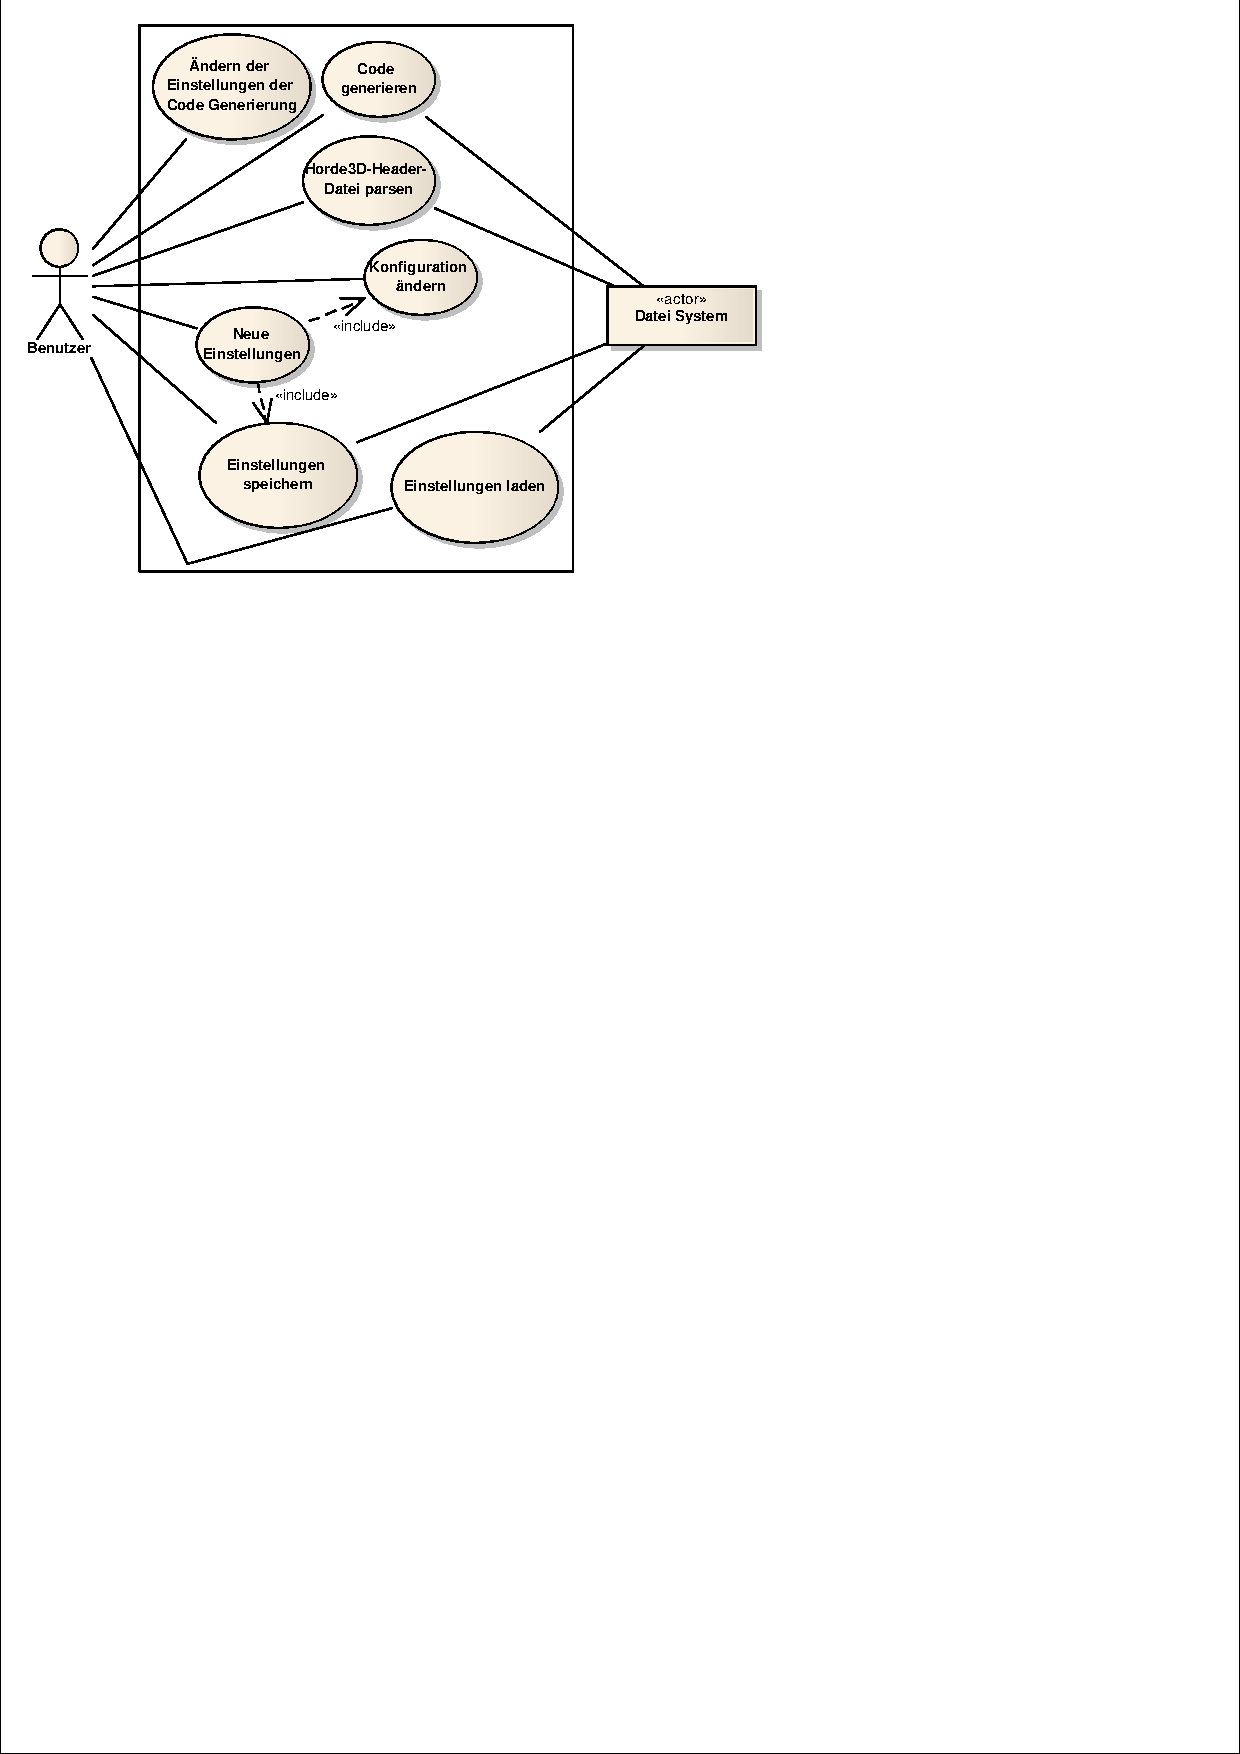
\includegraphics[trim = 1mm 200mm 80mm 1mm, clip, scale=0.7]{images/CodeGen_UseCaseModel.pdf}
\caption{Das \emph{Use Case} Modell des Code Generators}\label{fig:cgUCModel}
\end{figure}

Die im \emph{Use Case} Modell~\ref{fig:cgUCModel} gezeigten Anwendungsf�lle des Code Generators sind weitestgehend selbsterkl�rend. Mit dem System soll man die vorgenommenen Einstellungen speichern und sp�ter wieder laden k�nnen. Der Benutzer soll au�erdem den Namen der generierten Code-Dateien angeben k�nnen und auf Wunsch alle Einstellungen verwerfen und von vorne beginnen k�nnen. Interessanter sind die Anwendungsf�lle f�r das �ndern der Einstellungen der Code Generierung und f�r das Parsen der \emph{Header}-Datei. Ersteres wird durch das Aktivit�tsdiagramm~\ref{fig:cgChange} dargestellt. Wenn der Benutzer die Einstellungen �ndern m�chte, zeigt ihm das System zun�chst alle problematischen Funktionen an. In der Liste sind alle Funktionen, f�r die die Konvertierung mindestens eines Parameters oder des R�ckgabewertes problematisch ist. Auf Wunsch kann sich der Benutzer aber auch alle \Horde-Funktionen anzeigen lassen. Der Benutzer kann nun eine der Funktionen ausw�hlen, und das System zeigt die ausgew�hlten Typumwandlungen f�r alle Parameter und den R�ckgabetyp an. Problematische Konvertierungen werden hervorgehoben. Ein Konvertierungsproblem kann nun als gel�st markiert werden, oder die automatisch gew�hlte Umwandlung ge�ndert werden. Das System speichert die �nderungen, und der Benutzer kann weitere Einstellungen der gew�hlten Funktion oder weiterer Funktionen �ndern.

Beim Parsen der \emph{Header}-Datei von \Horde\ sollen alle Funktionen und ihre Parameter- und R�ckgabetypen ausgelesen werden. Es soll versucht werden, eine automatische Typumwandlung f�r alle Typen der Funktion zu finden. Gelingt dies nicht, soll die Umwandlung als problematisch markiert werden. Falls eine aktualisierte \emph{Header}-Datei geparst wird und der Benutzer vor dem Update bereits manuelle Einstellungen vorgenommen hat, sollen diese �bernommen werden. Es muss dazu f�r jede zuvor manuell ge�nderte Funktion �berpr�ft werden, ob die �nderungen auf die neu geparste Funktion �bertragen werden k�nnen. Sollte dies nicht gelingen, so soll die Funktion als problematisch markiert werden und die alten Einstellungen zus�tzlich zu den neu generierten gespeichert werden.

Abbildung~\ref{fig:cgDomain} zeigt das Konzeptmodell des Code Generators. \texttt{CodeGenerationSettings} speichert den Dateinamen der zu generierenden \C++- und \Csharp-Dateien, sowie eine Liste der \Horde-Funktionen. Die Einstellungen k�nnen in einer Datei gespeichert und wieder geladen werden. Der programmiersprachliche Aufbau der Funktionen wurden in seine Bestandteile zerlegt: Das \texttt{Function}-Konzept enth�lt den Funktionsnamen und hat f�r den R�ckgabetyp und alle Parameter der Funktion eine Assoziation zu einem \texttt{Type}-Konzept. Dort wird der \C++-Typ gespeichert und festgehalten, ob die Konvertierung problematisch ist, das Problem als gel�st markiert wurde oder ob vom Benutzer manuelle �nderungen vorgenommen wurden. Die gew�hlte Typumwandlung eines \texttt{Type}s wird durch die Assoziation zu einem Konzept der \texttt{TypeConversion}-Hierarchie beschrieben. Diese Hierarchie entspricht im wesentlichen den oben beschriebenen Kategorien der Typumwandlung. \texttt{ToStringConversion} macht aus einem \texttt{const char*} einen \texttt{System.String}, \texttt{ToEnumConversion} konvertiert eine \C++-Aufz�hlung in eine \Csharp-Aufz�hlung, bei einer \texttt{DirectConversion} bleibt der Typ unver�ndert, \texttt{DereferencePointerConversion} dereferenziert einen Zeiger und \texttt{CodeConversion} erlaubt beliebigen Code. Der Grund f�r diese genaue Aufschl�sselung der Konvertierungsmethoden liegt in dem unterschiedlichen Code begr�ndet, der f�r die jeweiligen Methoden generiert werden muss. Die \texttt{TypeConversion}-Hierarchie erlaubt f�r die Fallunterscheidungen virtuelle Funktionen zu verwenden, anstatt explizit mit \texttt{if-then-else}-Konstruktionen arbeiten zu m�ssen. Aufgrund dieser sehr implementierungsnahen Argumentation h�tte die Hierarchie auch erst in der Design- oder sogar erst in der Implementierungs-Phase eingef�hrt werden k�nnen. Da jedoch die unterschiedlichen Konvertierungskonzepte bereits in dieser Phase untersucht wurden und im Mittelpunkt der Anwendung stehen, wurden sie bereits ins Konzeptmodell aufgenommen.

Der \texttt{AutomaticTypeConverter} versucht �ber die ihm bekannten \texttt{ConversionRule}s f�r einen gegebenen \texttt{Type} die beste \texttt{TypeConversion} zu finden. Eine Umwandlungsregel kann als problematisch markiert sein, wenn ihre Richtigkeit nicht garantiert werden kann. Welche Regeln der Code Generator kennt und verwendet, wird in Abbildung~\ref{fig:cgRules} aufgelistet.

\subsection{Code Generator Phase II: Design}
Wie aus Abbildung~\ref{fig:cgDesign} ersichtlich ist, gibt es nur wenige Unterschiede zwischen dem Designmodell und dem Konzeptmodell des Code Generators. Die Verantwortlichkeiten wurden auf die Klassen verteilt und die \texttt{TypeConversion}-Hierarchie noch etwas verfeinert. Es wird nun zwischen der aus dem Konzeptmodell bekannten \texttt{CodeConversion} und den neuen \texttt{InlineConversion}s unterschieden. Au�er der \texttt{CodeConversion} erben alle anderen Konvertierungsklassen von der Basis-Klasse \texttt{InlineConversion}, da die jeweiligen Typumwandlungen in nur einer Zeile Code ausgef�hrt werden k�nnen. \texttt{CodeConversion} erlaubt im Unterschied dazu  beliebig langen Code �ber mehrere Zeilen, wohingegen \texttt{InlineCodeConversion} beliebigen Code in nur einer einzigen Zeile zul�sst.

Ebenfalls im Design hinzugekommen ist die Klasse \texttt{Horde3DHeaderFileParser}, welche die Funktionen in der \emph{Header}-Datei parst und in die Objekt-Struktur der Funktionen aufbaut.

Der Code f�r die Code Generierung wird aus den \texttt{Function}-Objekten ausgelagert. Diese Mischung aus \emph{Decorator} und \emph{Strategy Pattern} wird durch die \texttt{FunctionCodeGenerator}-Hierarchie umgesetzt. Abh�ngig von der Art des zu generierenden Codes wird jedes \texttt{Function}-Objekt an eine \texttt{C++FunctionGenerator}- oder \texttt{{\Csharp}FunctionGenerator}-Instanz �bergeben. Die Klassen enthalten die ben�tigten Funktionen zur Generierung des Codes und zum Anzeigen einer Code-Vorschau. Erstellt werden die \texttt{FunctionCodeGenerator}-Objekte durch eine \texttt{CodeGenerator}-Instanz, die Funktionen zur Generierung des gesamten Codes anbietet.

Einziges Modell des Code Generators ist die \texttt{CodeGenerationSettings}-Klasse, die im Designklassen-Diagramm mit dem Stereotyp \texttt{model} hervorgehoben wurde.

Die Abbildungen~\ref{fig:cgGetPFunc} und~\ref{fig:cgIsProb} zeigen die Vorgehensweise zur Ermittlung aller Funktionen mit problematischen Typ-Konvertierungen. Es werden alle Funktionen zur�ckgeliefert, f�r die die Umwandlung des R�ckgabetyps oder mindestens eines Parametertyps problematisch ist. Falls beim Aktualisieren der Funktion manuelle Benutzereingaben nicht automatisch �bernommen werden konnten, wird die Funktion ebenfalls zur�ckgeliefert.

Das Parsen der \emph{Header}-Datei wird durch das Sequenzdiagramm~\ref{fig:cgParse} dargestellt. Zun�chst wird eine Instanz der \texttt{Horde3DHeaderFileParser}-Klasse erzeugt und der Pfad zur \emph{Header}-Datei �bergeben. In der �bergebenen Datei werden alle Funktionen extrahiert und deren R�ckgabetyp und Parameter ermittelt. F�r alle Typen der Funktion wird die passende Typ\-umwandlung gesucht. Die \texttt{GuessTypeConversion}-Methode der \texttt{Type}-Klasse verwendet die \emph{Singleton}-Instanz des \texttt{AutomaticTypeConverter}s, um basierend auf dem \C++-Typen und den Konvertierungsregeln ein geeignetes \texttt{TypeConversion}-Objekt zu erzeugen. Nachdem f�r alle Funktionen alle ben�tigten Objekte erstellt wurden, wird versucht, alle manuellen �nderungen des Benutzers in die neuen Funktionsobjekte zu kopieren. Sollte es dabei zu Problemen kommen, wird das alte Funktionsobjekt mit all seinen Einstellungen �ber die \texttt{OldFunction}-Assoziation mit dem neuen Funktionsobjekt verbunden. Die Funktion wird dann als problematisch gelistet, und der Benutzer kann seine �nderungen �berpr�fen und nachziehen.

\subsection{Code Generator Phase III: Implementierung}\label{cgImpl}
W�hrend der Implementierung des Code Generators erwies sich die hierarchische Einteilung der \texttt{TypeConversion} als vorteilhaft. Der Code zum Generieren des \Csharp-Codes konnte mit Ausnahme der \texttt{ToEnumConversion} komplett durch die abstrakte \texttt{TypeConversion}-Klasse selbst abgedeckt werden. Bei der Umsetzung der Generierung des \C++-Codes hingegen gab es gr��ere Unterschiede. Durch die Verwendung virtueller Funktionen konnte der Code jedoch auf die einzelnen \texttt{TypeConversion}-Klassen aufgeteilt werden, wodurch die \texttt{FunctionCodeGenerator}-Klassen keine Fallunterscheidungen auf Grundlage der verwendeten Typ-Konvertierungen durchf�hren m�ssen.

\begin{figure}[htp]
\centering
%trim=l b r t  	This option will crop the imported image by l from the left, b from the bottom, r from the right, and t  from the top. Where l, b, r and t are lengths. 
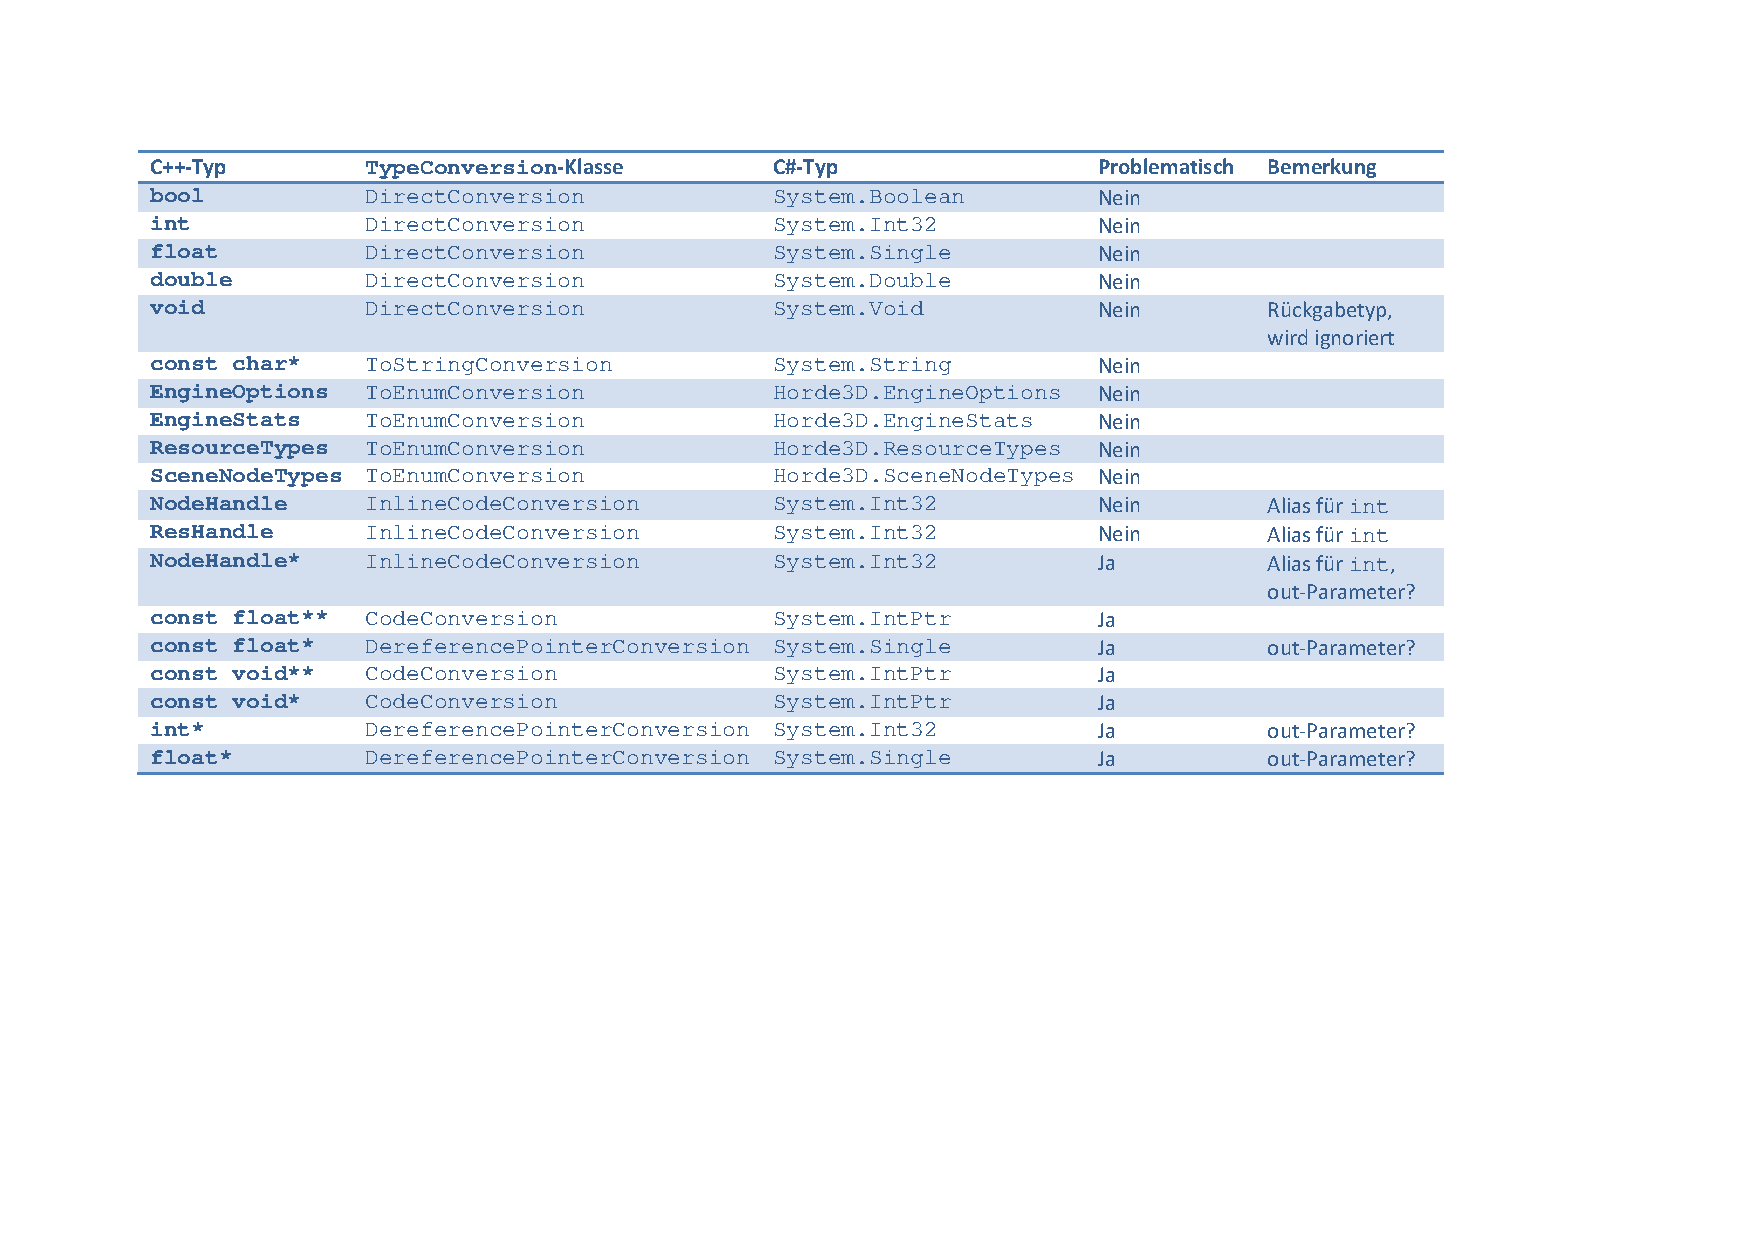
\includegraphics[trim = 20mm 75mm 55mm 20mm, clip, scale= 0.7]{images/CodeGen_Rules.pdf}
\caption{Konvertierungsregeln des Code Generators}\label{fig:cgRules}
\end{figure}	

F�r das Parsen der Funktionen in der \Horde-\emph{Header}-Datei wurden \emph{Regular Expressions} verwendet, wodurch der Parsing-Code kompakt gehalten werden konnte. Auch f�r die Generierung des \Csharp-Codes wurde auf bereits vorhandene .NET-Funktionalit�ten zur�ckgegriffen; .NET enth�lt einen Code Generator f�r \Csharp, Visual Basic .NET und \C++/CLI. Der \C++-Code musste jedoch von Hand durch Konstruktion eines Strings generiert werden, da der .NET Code Generator keinen nativen \C++-Code erzeugen kann.

Die Bestimmung der ben�tigten \texttt{CodeConversionRule}s orientierte sich an den verwendeten Datentypen der \Horde-Funktionen und ist somit nicht allgemein vollst�ndig, sondern nur ausreichend f�r Version 1.0.0 Beta 3 von \Horde. Die Konvertierungsregeln sind in Abbildung~\ref{fig:cgRules} tabellarisch aufgelistet.

%\begin{sidewaystable}[htp]
%	\centering
%		\begin{tabular}{|l|l|l|l|p{3.5cm}|}
%		  \hline
%		  \multicolumn{5}{|c|}{\textbf{Konvertierungsregeln des Code Generators}} \\
%			\hline
%			\C++-Typ & \texttt{TypeConversion}-Klasse & \Csharp-Typ & Problematisch & Bemerkung\\
%			\hline
%			\texttt{bool} & \texttt{DirectConversion} & \texttt{System.Boolean} & nein & \\
%			\texttt{int} & \texttt{DirectConversion} & \texttt{System.Int32} & nein & \\
%			\texttt{float} & \texttt{DirectConversion} & \texttt{System.Single} & nein & \\
%			\texttt{double} & \texttt{DirectConversion} & \texttt{System.Double} & nein & \\
%			\texttt{void} & \texttt{DirectConversion} & \texttt{System.Void} & nein & R�ckgabe-Typ, wird ignoriert\\
%			\texttt{const char*} & \texttt{ToStringConversion} & \texttt{System.String} & nein & \\
%			\texttt{EngineOptions} & \texttt{ToEnumConversion} & \texttt{Horde3D.EngineOptions} & nein & \\
%			\texttt{EngineStats} & \texttt{ToEnumConversion} & \texttt{Horde3D.EngineStats} & nein & \\
%			\texttt{ResourceTypes} & \texttt{ToEnumConversion} & \texttt{Horde3D.ResourceTypes} & nein & \\
%			\texttt{SceneNodeTypes} & \texttt{ToEnumConversion} & \texttt{Horde3D.SceneNodeTypes} & nein & \\
%			\texttt{NodeHandle} & \texttt{InlineCodeConversion} & \texttt{System.Int32} & nein & Alias f�r \texttt{int} \\
%			\texttt{ResHandle} & \texttt{InlineCodeConversion} & \texttt{System.Int32} & nein & Alias f�r \texttt{int}\\
%			\texttt{NodeHandle*} & \texttt{InlineCodeConversion} & \texttt{System.Int32} & ja & Alias f�r \texttt{int}, out-Parameter? \\
%			\texttt{const float**} & \texttt{CodeConversion} & \texttt{System.IntPtr} & ja & \\
%			\texttt{const float*} & \texttt{DereferencePointerConversion} & \texttt{System.Single} & ja & out-Parameter? \\
%			\texttt{const void**} & \texttt{CodeConversion} & \texttt{System.IntPtr} & ja & \\
%			\texttt{const void*} & \texttt{CodeConversion} & \texttt{System.IntPtr} & ja & \\
%			\texttt{int*} & \texttt{DereferencePointerConversion} & \texttt{System.Int32} & ja & out-Parameter? \\
%			\texttt{float*} & \texttt{DereferencePointerConversion} & \texttt{System.Single} & ja & out-Parameter? \\
%			\hline
%			\end{tabular}
%\end{sidewaystable}		

\subsection{Code Generierung nach einem Update der Horde3D-API}
Wenn sich die �ffentliche API einer neuen \Horde-Version ge�ndert hat, muss die Code Generierung erneut ausgef�hrt werden. Um �nderungen, die an den Einstellungen problematischer Funktionen durchgef�hrt wurden, nicht immer wieder machen zu m�ssen, verf�gt der Code Generator �ber einen automatischen Update-Mechanismus. Tabelle~\ref{fig:cgStats} zeigt, wie dieser Mechanismus mit API-Updates zurechtkommt.

%\begin{table}[ht]
%	\centering
%		\begin{tabular}{|p{5.5cm}|l|l|l|l|}
%		  \hline
%		  & \multicolumn{4}{|c|}{\Horde\ Version} \\
%			\hline
%			& 0.0.15 & 1.0.0 Beta 1 & 1.0.0 Beta 2 & 1.0.0 Beta 3 \\
%			\hline
%			\Horde-Funktionen & 67 & 68 & 75 & 78 \\
%			Problematische Funktionen & 9 & 9 & 10 & 10 \\
%			~~~~... bereits als gel�st markiert & - & 9 & 9 & 9 \\
%			~~~~... eigentlich unproblematisch & 3 & 0 & 1 & 0 \\
%			Notwendige �nderungen & 6 & 0 & 0 & 1 \\
%			�nderungen �bernommen & - & 6 & 9 & 9 \\
%			�nderungen verworfen & - & 0 & 0 & 1 \\
%			\hline
%			\end{tabular}
%			\caption{�bersicht �ber die �bernahme von �nderungen an problematischen Funktionen nach einem Update der \Horde-API}\label{tab:updateStats}
%\end{table}		

\begin{figure}[htp]
\centering
%trim=l b r t  	This option will crop the imported image by l from the left, b from the bottom, r from the right, and t  from the top. Where l, b, r and t are lengths. 
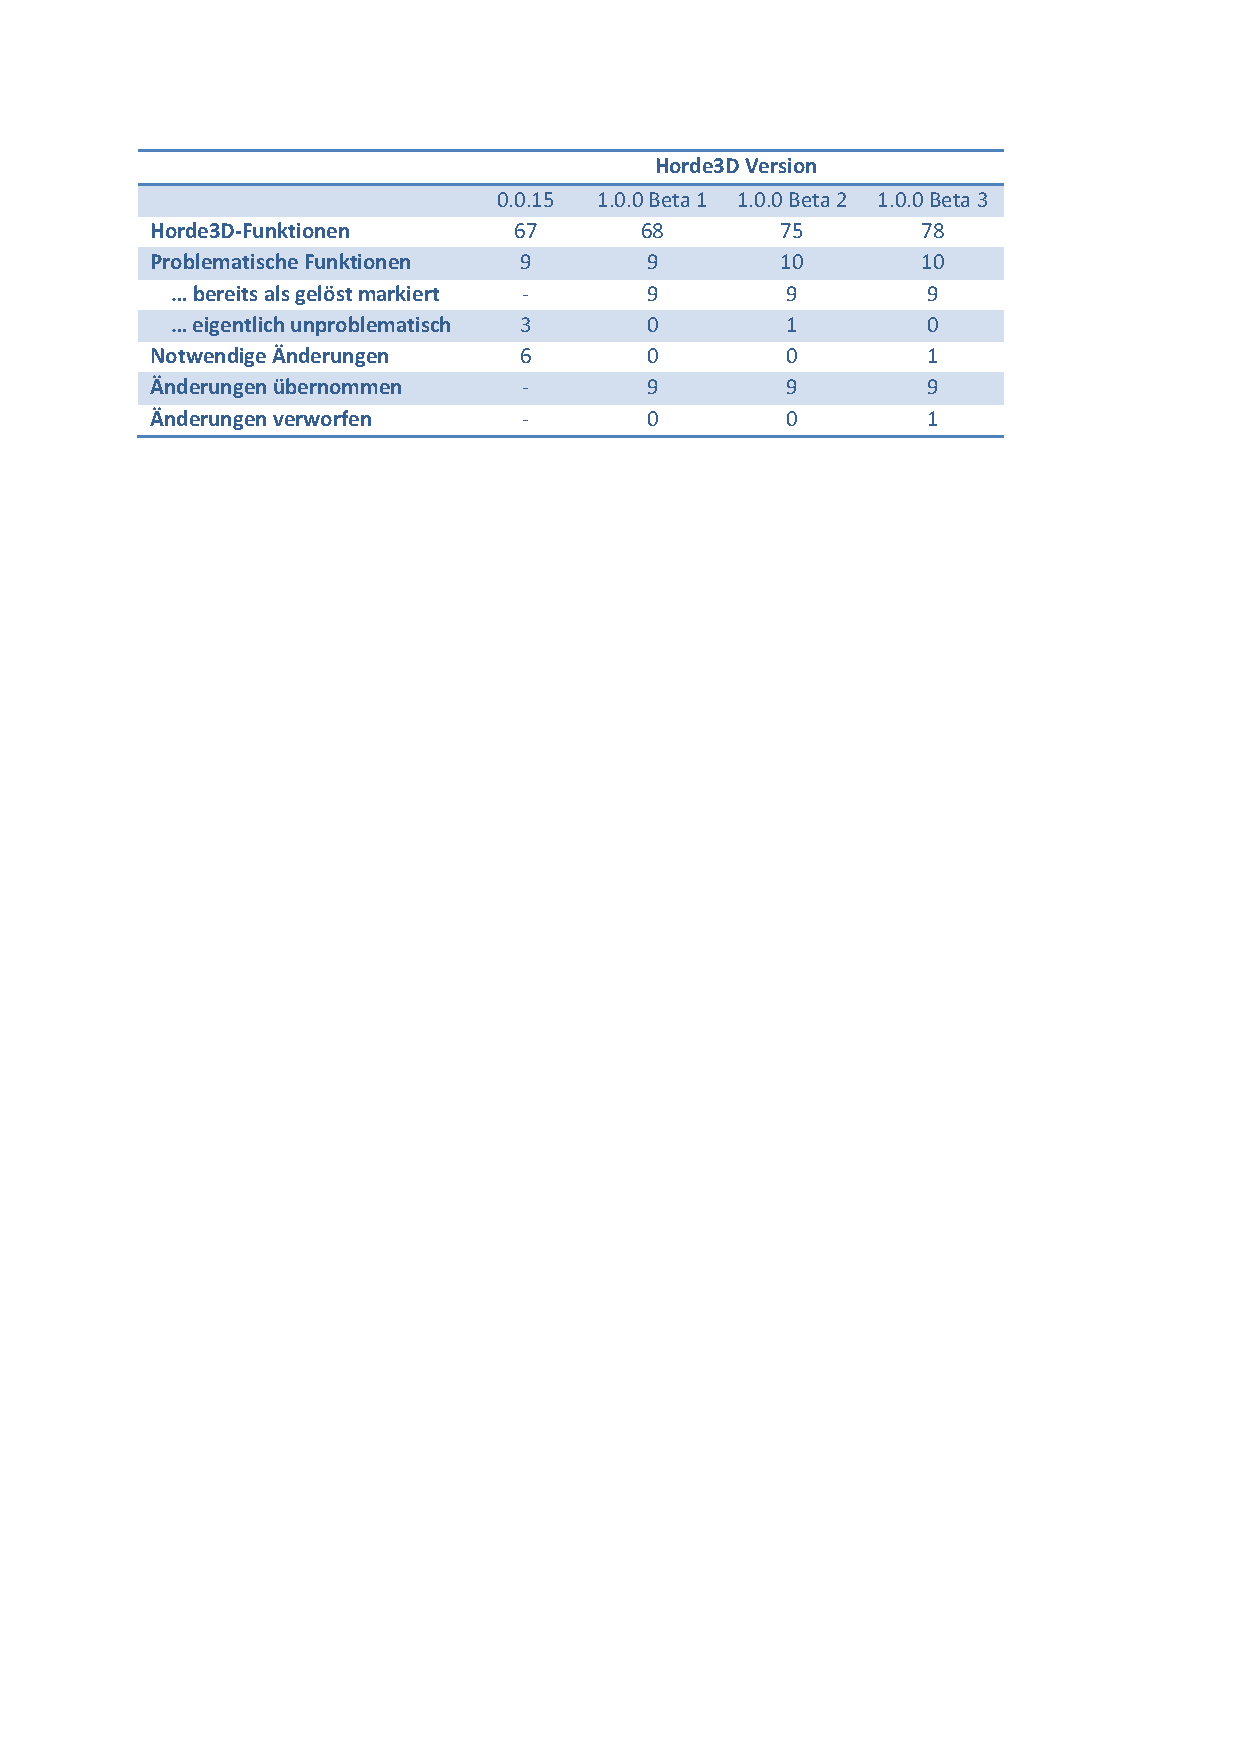
\includegraphics[trim = 20mm 220mm 20mm 20mm, clip, scale = 0.7]{images/CodeGen_Stats.pdf}
\caption{Evaluation des Update-Mechanismus des Code Generators}\label{fig:cgStats}
\end{figure}	

Ausgehend von Version 0.0.15 wurden die API-Updates auf die Betas 1, 2 und 3 von \Horde\ 1.0.0 untersucht. Version 0.0.15 hatte 67 �ffentliche Funktionen, von denen neun als problematisch markiert wurden. Von diesen neun waren wiederum drei eigentlich unproblematisch. Die Annahme, bei Zeiger-Parametern handle es sich eigentlich um \emph{out}-Parameter, war f�r diese drei Funktionen korrekt. Die verbleibenden sechs problematischen Funktionen mussten allerdings wirklich von Hand modifiziert werden. In zwei F�llen konnten \texttt{void}-Zeiger sogar nur als \texttt{System.IntPtr} weitergereicht werden. Ansonsten war es m�glich, \texttt{float}-Zeiger, die Matrizen repr�sentierten, als \texttt{float}-\emph{Arrays} der L�nge 16 weiterzugeben.

Beim Update auf Version 1.0.0 Beta 1 kam eine neue, unproblematische Funktion hinzu. Die manuellen �nderungen konnten alle erfolgreich �bernommen werden, sodass nichts weiter zu tun war und der Code sofort neu generiert werden konnte. Mit Beta 2 kamen weitere Funktionen hinzu, von denen eine als problematisch erkannt wurde. Allerdings war auch hier die \emph{out}-Parameter-Annahme korrekt. Alle manuellen �nderungen von Version 0.0.15 wurden auch bei diesem Update korrekt �bernommen. Beta 3 f�hrte weitere neue Funktionen ein. Beim Update wurde allerdings eine manuelle �nderung verworfen, da die Funktion umbenannt wurde. Umbenannte Funktionen erkennt der Update-Mechanismus nicht. Die �nderung musste also manuell aus den vorherigen Einstellungen kopiert werden; ansonsten waren aber auch in diesem Update-Schritt keine weiteren Anpassungen n�tig.
\section{Client-Server-Kommunikation}
Bei der Implementierung der Client-Server-Kommunikation mit der Windows Communication Foundation konnte das \texttt{IDebuggerService}- und das \texttt{IDebuggerServiceCallback}-Interface aus dem Design unver�ndert �bernommen werden. Aus technischen Gr�nden musste allerdings noch die Service-Operation \texttt{RegisterClient} hinzugef�gt werden. Der Client ruft diese Funktion sofort nach dem Zustandekommen der Verbindung auf, um seinen \emph{Callback Channel} beim Server zu registrieren. Dann erst kann der Server \emph{Callbacks} an den Client schicken.

Es mussten besondere Ma�nahmen getroffen werden, um \emph{Deadlocks} und \emph{Race Conditions} zu vermeiden. Die \Horde-Anwendung kann mehrere Threads verwenden; der Server hat keine M�glichkeit dies herauszufinden und sollte davon auch nicht abh�ngen, da die \Horde-API sowieso nicht \emph{thread-safe} ist. Die Implementierung geht deshalb davon aus, dass alle \Horde-Funktionen vom gleichen Thread aus aufgerufen werden. WCF f�hrt aber jede Anfrage des Clients in einem gerade zur Verf�gung stehenden Thread des \emph{Thread Pools} aus. Da die Service-Operationen zumindest teilweise auf \Horde-Funktionen zugreifen, k�nnte es somit zu \emph{Race Conditions} kommen oder auf inkonsistenten Zust�nden gearbeitet werden. Es musste daher sichergestellt werden, dass jeder Server-Aufruf im gleichen Thread wie \Horde\ l�uft. 

Das .NET Framework bietet die \texttt{SynchronizationContext}-Klasse f�r Threadwechsel an. Der \texttt{Post}-Methode dieser Klasse kann ein \emph{Delegate} �bergeben werden, der in einem ganz bestimmten Thread ausgef�hrt wird. Leider stellt die Standard-Implementierung der Klasse nur die Funktionen bereit, das Wechseln des Threads ist nicht implementiert\footnote{Der Grund daf�r ist, dass es verschiedene M�glichkeiten f�r die Implementierung des Threadwechsels gibt. .NET bietet zwei Implementierungen f�r WinForms und WPF an, die allerdings auch nur von WinForms- und WPF-Anwendungen verwendet werden k�nnen. \Horde-Anwendung k�nnen aber auch die native Win32-API zum Erzeugen des Anwendungsfensters benutzen.}. Es wurde daher der \texttt{Horde3DSynchronizationContext} entwickelt, der von \texttt{SynchronizationContext} erbt. Wird die \texttt{Post}-Methode der Klasse aufgerufen, wird die �bergebene Funktion in einer \texttt{Queue} \emph{thread-safe} protokolliert, aber noch nicht ausgef�hrt. 

Bei jedem Aufruf einer \Horde-Funktion l�st \texttt{Horde3DCall} das \texttt{BeforeFunctionCalled}-Ereignis aus. Der \texttt{Horde3DDebugger} registriert einen \emph{Event Handler}, der beim Ausl�sen dieses Ereignisses die \texttt{Execute}-Methode des \texttt{Horde3DSynchronizationContext}s aufruft. Da die Horde-Funktion und somit auch das Ereignis im \Horde-Thread laufen, werden alle Methoden, die derzeit in der \texttt{Queue} des Synchronisationskontexts liegen, der Reihe nach im \Horde-Thread ausgef�hrt.

Dieses Prinzip stellt sicher, dass alle Aufrufe der WCF-Serverfunktionen im \Horde-Thread laufen. Da WCF sehr flexibel und konfigurierbar entwickelt wurde, kann WCF automatisch eine Instanz des \texttt{Horde3DSynchronizationContext}s zum Wechseln des Threads verwenden. Dazu musste das \texttt{Horde3DThreadAffinityAttribute}-Attribut definiert werden, welches das \texttt{IContractBehavior}-Interface von WCF implementiert. Mit diesem Attribut kann der Synchronisationskontext von WCF programmatisch gesetzt werden \cite{wcf}.

Das Design sah auch vor, dass \emph{Callback}-Aufrufe garantiert an den Client geschickt werden, auch, wenn dieser noch gar nicht verbunden ist. Die \texttt{DebuggerService}-Klasse wurde daher um statische Funktionen f�r jede \emph{Callback}-Operation erweitert, die den \emph{Callback}-Aufruf abfangen und in einen anderen Thread verlagern. Dieser Thread versucht solange den \emph{Callback} auszuf�hren, bis eine Verbindung aufgebaut wurde und der \emph{Callback} erfolgreich durchgef�hrt werden konnte.

Client-seitig werden Serveroperationen immer aus einem \emph{Backgroundthread} aufgerufen, damit die GUI nicht blockiert wird und weiterhin auf Benutzereingaben reagieren kann. Die \texttt{DebuggerServiceProxy}-Klasse k�mmert sich intern um die Verbindung zum Server und die Thread-Verwaltung. Falls der Client noch nicht zum Server verbunden ist, wird vor dem Aufruf der Operation eine Verbindung aufgebaut.

Ein Problem ergab sich durch die Assoziationen zwischen den Ressourcen und insbesondere der \emph{Scene Nodes} untereinander. WCF serialisiert immer den kompletten Objektgraph. Schickt man also beispielsweise einen \emph{Scene Node} an den Client, wird auch dessen Vaterknoten mitgeschickt. Aber auch der Vater des Vaters wird mit �bertragen. Das endet erst beim Erreichen der Wurzel. Um dieses Problem zu vermeiden, werden die Assoziationen �ber die \texttt{NodeHandle}s beziehungsweise \texttt{ResHandle}s identifiziert. Der Client muss dann �ber diese IDs das eigentliche Objekt beim \texttt{SceneGraph}- oder \texttt{ResourceGraph}-Modell erfragen. Die Zuordnung von den IDs zu den Objekten erfolgt �ber eine Hashtabelle, hat also nur die Komplexit�t $O(1)$. Um den Zugriff syntaktisch m�glichst einfach zu halten, ist in der \texttt{Graph}-Klasse ein Indexoperator definiert. Das folgende Beispiel zeigt die Implementierung des \emph{Properties} \texttt{SceneNode.Parent}, das �ber die \texttt{SceneGraph}-Instanz und den \texttt{NodeHandle} des Vaters die Vater-Instanz zur�ckliefert:

\lstset{language=Java} 
\begin{lstlisting}
public class SceneNode
{
	internal int ParentHandle { get; }
	
	public SceneGraph SceneGraph { get; set; }
	
	public SceneNode Parent
	{
		get { return SceneGraph[ParentHandle]; }
	}
	
	// ...
}
\end{lstlisting}

Der Zugriff auf die Vater-Instanz �ber das \texttt{ParentHandle}-\emph{Property} wird komplett gekapselt. F�r den Benutzer der Klasse macht es keinen Unterschied, ob die Vater-Instanz direkt �bertragen wird, oder aus dem \texttt{SceneGraph}-Objekt stammt.
\section{Anhalten der Anwendung}\label{suspendApp}
Das \DevEnv\ verwendet drei verschiedene Implementierungen des \texttt{ISuspendApplicationStrategy}-Interfaces zum Anhalten der Anwendung. Eine Strategie t�uscht dem Prozess vor, dass keine Zeit mehr vergeht. Eine andere leitet alle Tastatur- und Mauseingaben des Benutzers an eine andere Funktion um. Die dritte Klasse zum Fangen und Freilassen des Mauszeigers kam erst nach der zweiten Iteration der Design-Phase hinzu. Dank der Verwendung des \emph{Strategy Patterns} musste jedoch nur eine Zeile Code im Konstruktor der \texttt{SuspendApplicationStrategy}-Klasse hinzugef�gt werden, um die dritte Strategie einzubinden.

Die urspr�ngliche Idee war, den Prozess der Anwendung wirklich anzuhalten. Dazu gibt es die Funktionen \texttt{SuspendThread} und \texttt{ResumeThread} der Win32-API. Mit Hilfe dieser Funktionen kann ein Thread pausiert und wieder fortgesetzt werden. Ruft man diese Funktionen f�r alle Threads eines Prozesses auf, so wird der komplette Prozess eingefroren und wieder fortgesetzt. Dieses Verfahren ist jedoch nicht problemlos anwendbar, da Teile des Prozesses noch weiterlaufen sollten; so sollte WCF in der Lage sein, Anfragen vom Client zu bearbeiten und \emph{Callbacks} auszul�sen. Um das zu gew�hrleisten, darf der Thread, in dem WCF l�uft, nicht angehalten werden. Die Win32-Funktionen arbeiten aber auf nativen Threads, w�hrend WCF in einem \emph{managed} Thread l�uft. Es kann aber passieren, dass die CLR mehrere \emph{managed} Threads im gleichen nativen Thread laufen l�sst. Noch problematischer wird es, wenn die \Horde-Anwendung ebenfalls in .NET geschrieben wurde oder mehrere \emph{AppDomains}\footnote{Eine .NET-\emph{AppDomain} kann man sich als einen .NET-Prozess vorstellen. Es kann in einem nativen Prozess mehrere \emph{AppDomains} geben. Das Betriebssystem kennt das Konzept der \emph{AppDomains} nicht.} im Prozess laufen. Es ist also schwierig genau festzustellen, welche Threads angehalten werden d�rfen. Des Weiteren kommt noch hinzu, dass es verschiedene Versionen der \texttt{Suspend-/ResumeThread}-Funktionen f�r native 32 Bit Prozesse, 32 Bit Prozesse unter einem 64 Bit Betriebssystem und 64 Bit Prozesse gibt.

Derzeit ist f�r das richtige Anhalten des Prozesses keine \texttt{ISuspendApplicationStrategy}-Implementierung vorhanden. In vielen F�llen sind die drei im folgenden vorgestellten Strategien ausreichend. Es gibt aber auch F�lle, in denen ein richtiges Anhalten des Prozesses notwendig w�re. Im folgenden Abschnitt wird auf diese Problematik n�her eingegangen.

\subsection{Anhalten der Zeit}\label{stoptime}
Um den Prozess nicht wirklich anhalten zu m�ssen, wurde eine Idee aus NVIDIAs PerfHUD �bernommen: Das Anhalten der Zeit. Im Benutzerhandbuch gibt es einen Hinweis darauf, wie NVIDIA dieses Problem l�st: 

\begin{quote}"`PerfHUD �freezes� your application by returning the same value every time your application asks for the current time."' \cite[S. 11]{perfhud}\end{quote}

Das ist auch die Vorgehensweise des \DevEnvs. Die meisten Anwendungen verwenden die hochaufl�sende \emph{Timer}-Funktion \texttt{QueryPerformanceCounter}, um die vergangene Zeit zu messen. Jeder Aufruf dieser Funktion wird an eine Funktion des Servers umgeleitet. Dort wird der wirkliche \emph{Timer} aufgerufen und der R�ckgabewert aufgezeichnet. Ist die Anwendung angehalten, wird immer der Zeitwert zum Zeitpunkt des Anhaltens der Anwendung zur�ckgeliefert; die Anwendung meint, es sei seit dem letzten Frame keine Zeit vergangen. Dadurch ist die Zeit angehalten und die Anwendung pausiert. Wird die Anwendung wieder fortgesetzt, so wird wieder der richtige Zeitwert geliefert, abz�glich der Zeitdauer, w�hrend der die Anwendung pausiert war.

\begin{figure}[ht]
\centering
%trim=l b r t  	This option will crop the imported image by l from the left, b from the bottom, r from the right, and t  from the top. Where l, b, r and t are lengths. 
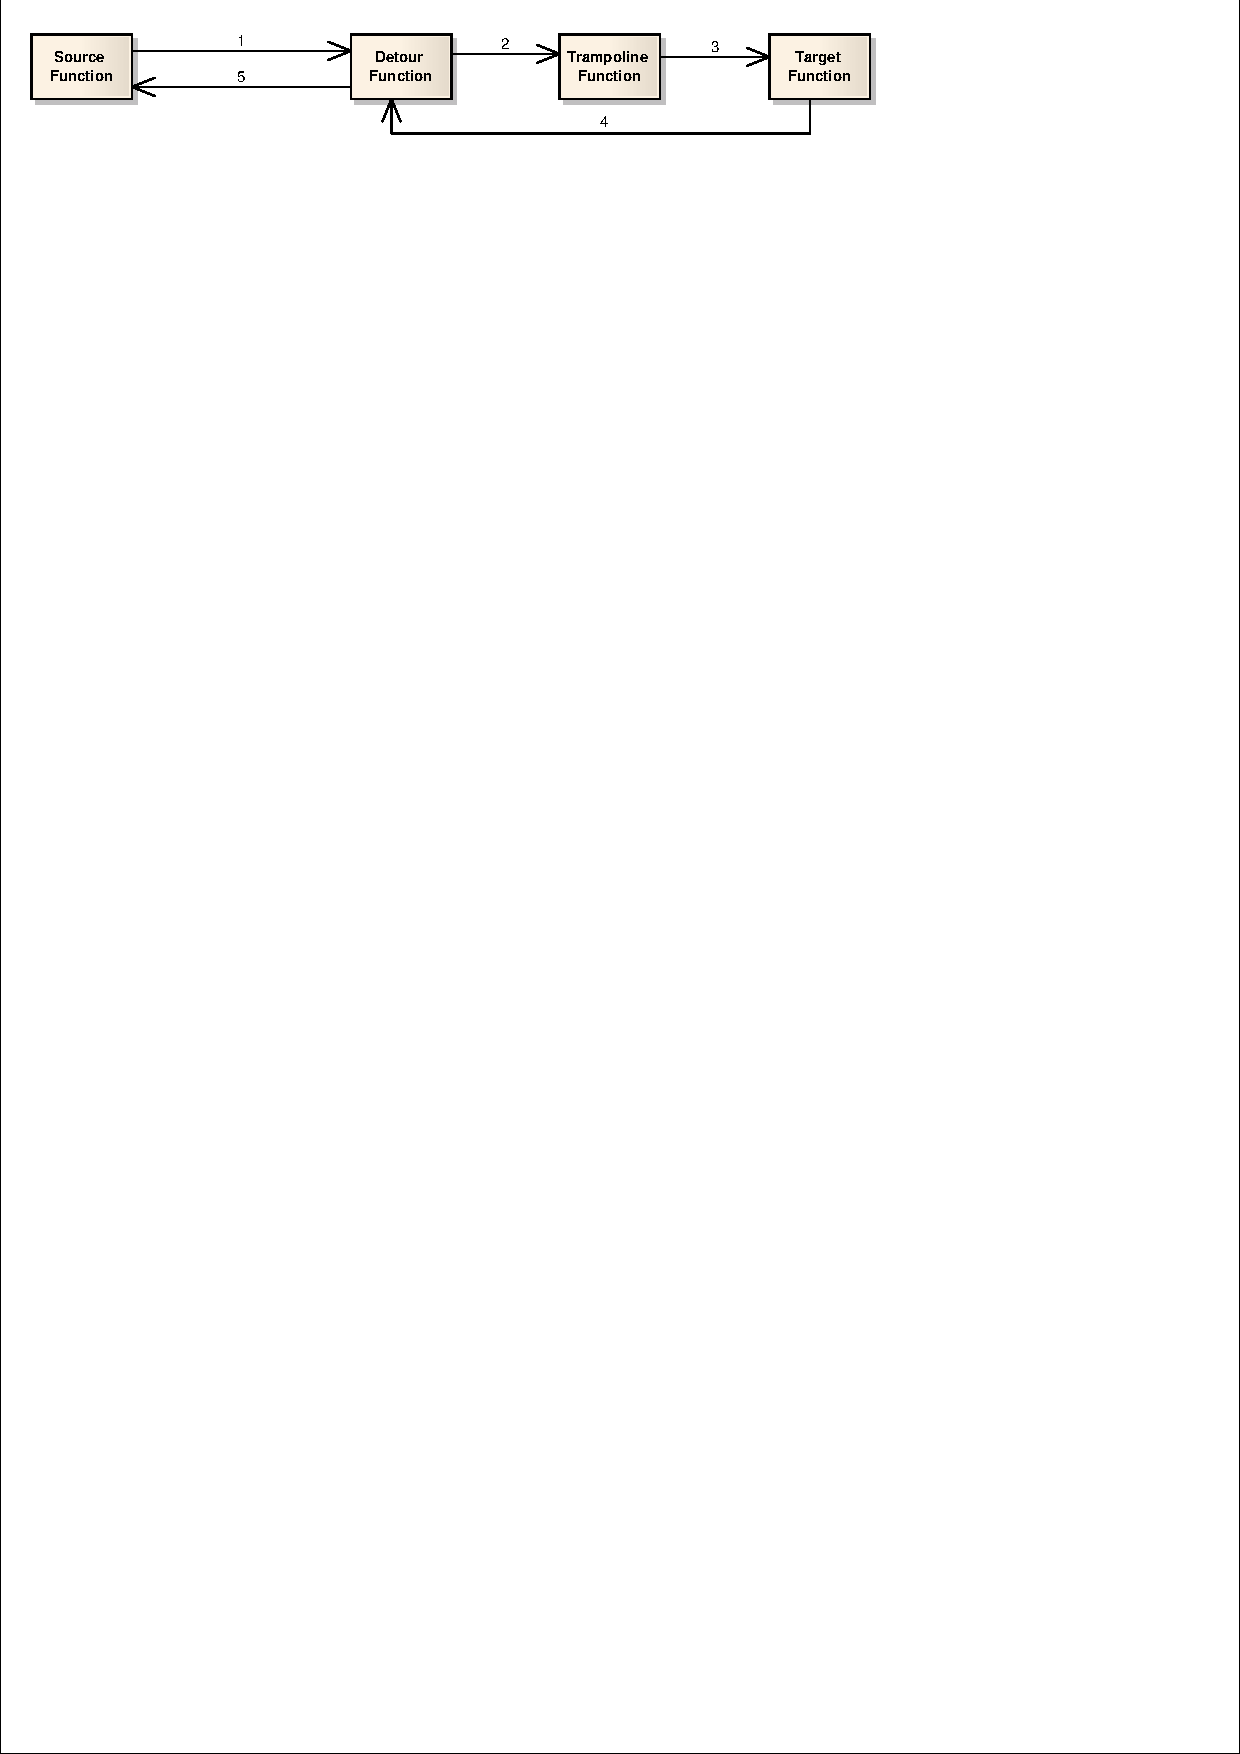
\includegraphics[trim = 5mm 270mm 60mm 5mm, clip, scale=0.7]{images/Detours.pdf}
\caption{Kontrollfluss bei einem abgefangenen Funktionsaufruf}\label{fig:detours}
\end{figure}

Technisch wird das Umleiten des Funktionsaufrufs durch Microsofts Detours Express Bibliothek gel�st. Die Bibliothek kann in einer Anwendung verwendet werden, um einen Aufruf einer beliebigen, nativen Funktionen (\emph{Target Function}) abzufangen und auf eine beliebige selbst definierte Funktionen (\emph{Detour Function}) umzuleiten. Zur Laufzeit schreibt Detours das Abbild des in den Prozess geladenen Bin�rcodes der \emph{Target Function} um. Abbildung~\ref{fig:detours} zeigt den Kontrollfluss beim abgefangenen Aufruf der \emph{Target Function}. Die ersten Instruktionen der \emph{Target Function} werden durch einen Sprung zur \emph{Detour Function} ersetzt. Es wird also als erstes die \emph{Detour Function} ausgef�hrt. Dort kann beliebiger Code abgearbeitet werden. Detours erzeugt au�erdem eine \emph{Trampoline Function}, welche die ersetzen Instruktionen der \emph{Target Function} enth�lt und anschlie�end zur \emph{Target Function} zur�ckspringt. Die \emph{Detour Function} kann die \emph{Trampoline Function} aufrufen, um die \emph{Target Function} auszuf�hren. Verl�sst der Kontrollfluss die \emph{Target Function}, ist wieder die \emph{Detour Function} aktiv und kann weiterhin beliebigen Code ausf�hren. Schlie�lich kehrt der Kontrollfluss zur aufrufenden Funktion (\emph{Source Function}) zur�ck.

Das Anhalten der Zeit hat einige wichtige Konsequenzen: Zum einen funktioniert die Vorgehensweise gar nicht, wenn die Anwendung nicht \texttt{QueryPerformanceCounter} zum Messen der Zeit verwendet. Da es aber keine anderen hochaufl�senden Zeitmesser f�r Windows gibt, wird dies nicht oft der Fall sein. Zum anderen kommt es zu Problemen, wenn die Anwendung nicht so schnell arbeitet wie sie kann, sondern auf eine gewisse Zahl an Updates pro Sekunde festgelegt ist. Falls die Anwendung beispielsweise maximal 60 mal pro Sekunde ein Update ausf�hrt, aber scheinbar seit dem letzten Frame keine Zeit vergangen ist, wird sie einfach gar nichts mehr tun; sie sollte aber wenigstens noch \texttt{Horde3D::render} aufrufen. Gegebenenfalls muss zur Verwendung des \DevEnvs\ die Frameraten-Limitierung abgeschaltet werden. Da beim Starten der Anwendung Kommandozeilenparameter �bergeben werden k�nnen, kann die Abschaltung der Limitierung prinzipiell auch ohne eine �nderung der Anwendung erfolgen, falls die Anwendung per Kommandozeile entsprechend konfigurierbar ist.

Das Vorgehen funktioniert auch nicht, wenn f�r zeitabh�ngige Berechnungen nicht die vergangene Zeit ${\Delta}t$ sondern die aktuellen \emph{Frames Per Second} (FPS) verwendet werden. Da FPS $= 1 / {\Delta}t$ wird die FPS-Berechnung f�r ${\Delta}t = 0$ entweder nicht ausgef�hrt, oder sie liefert keinen vern�nftigen Wert zur�ck.

Die Methode hat auch keinen Erfolg, wenn die Anwendung oder Teile der Anwendung zeitunabh�ngig arbeiten. Denkbar w�re zum Beispiel eine Client-Server-Anwendung, in der der Server kontinuierlich neue Positionen der Objekte berechnet und an den Client schickt. Der Client empf�ngt die Nachrichten des Servers, baut die Szene entsprechend um und zeichnet sie neu. F�r den Benutzer scheint die Anwendung weiterhin zu laufen, obwohl der Client eigentlich angehalten ist und f�r ihn keine Zeit mehr vergeht.

All diese Probleme w�rden nicht auftauchen, wenn der Prozess der Anwendung wirklich angehalten werden w�rde, wie oben beschrieben. Es wurde dennoch aus zwei Gr�nden nur die Zeit-Methode umgesetzt: Erstens ist wie beschrieben beim Anhalten des Prozesses nicht klar, welche Threads angehalten werden d�rfen, wohingegen die Implementierung der Zeit-Methode einfach ist. Zweitens wird die Zeit-Methode in jedem Fall ben�tigt. H�lt man die Threads der Anwendung an, so laufen diese zwar nicht weiter, die Zeit aber schon. Setzt man nun die Threads fort, so k�nnen seit dem letzten Frame mehrere Sekunden oder Minuten vergangen sein. Die Physik- und Animationssysteme rechnen dann mit einem viel zu gro�en ${\Delta}t$ von mehreren Sekunden oder Minuten und k�nnen eventuell keinen stabilen Zustand mehr erreichen.

\subsection{Ersetzen des Window Procedures}
Die Win32-API verwendet Nachrichten, um mit einem Anwendungsprozess zu kommunizieren. Mit den Nachrichten kann die Anwendung �ber alle wichtigen Ereignisse informiert werden: Mausklicks, Tastatureingaben, Mausbewegungen, Schlie�en der Anwendung, Verschieben des Anwendungsfensters, Ablaufen eines \emph{Timers}, und so weiter. Alle Nachrichten an einen Prozess beziehungsweise an ein Fenster werden an eine ausgewiesene Funktion, das \emph{Window Procedure} (\emph{WndProc}), geschickt. Dort wird als Reaktion auf spezielle Nachrichten anwendungsspezifischer Code ausgef�hrt.

Das \DevEnv\ muss auf zwei Arten mit dem \emph{Window Procedure} der Anwendung interagieren: Einerseits muss es Nachrichten abfangen, die f�r den Server eine Bedeutung haben. Dr�ckt der Benutzer beispielsweise die Taste F7, so soll der Server die Anwendung anhalten. Auf der anderen Seite darf das \emph{Window Procedure} der Anwendung keine Benutzereingaben mehr erhalten, wenn die Anwendung angehalten ist. Es soll aber dennoch m�glich sein, das Anwendungsfenster zu verschieben oder zu schlie�en. 

Bei der Initialisierung des Servers wird mit der Win32-Funktion \texttt{SetWindowsHookEx} ein prozessweiter \emph{Hook} aktiviert, der alle Nachrichten an das \emph{WndProc} der Anwendung abf�ngt. Innerhalb des \emph{Hooks} wird �berpr�ft, ob f�r den Server eine relevante Nachricht -- also zum Beispiel \texttt{KeyDown} f�r die Taste F7 -- geschickt wurde. In diesem Fall reagiert der Server entsprechend. Anschlie�end wird die Nachricht an das \emph{WndProc} weitergeleitet.

Mit der Funktion \texttt{SetWindowLongPtr} kann der \emph{WndProc}-Zeiger eines Fensters auf eine beliebige benutzerdefinierte Funktion gesetzt werden. Der Server ersetzt das \emph{Window Procedure} des Anwendungsfensters, wenn die Anwendung angehalten wird. Das \emph{WndProc} des Servers ignoriert alle eingehenden Nachrichten �ber Maus- und Tastatureingaben und behandelt nur Fenster-Nachrichten wie Verschieben oder Schlie�en. Beim Fortsetzen der Anwendung wird der Zeiger wieder auf das urspr�ngliche \emph{WndProc} gesetzt.

\subsection{Freigabe des Mauszeigers}
Viele Anwendungen beschr�nken den Mauszeiger auf ihre Fenstergr��e und verstecken ihn. Beim Testen des \DevEnvs\ mit den Beispielapplikationen des \Horde-SDKs zeigten sich verschiedene Probleme mit dieser exklusiven Benutzung der Maus. Der Server f�ngt daher -- wiederum mit der Detours Express Bibliothek von Microsoft -- alle Aufrufe der Win32-Funktionen \texttt{ShowCursor}, \texttt{ClipCursor} und \texttt{SetCursorPos} ab. Aufrufe dieser Funktionen werden protokolliert und anschlie�end die urspr�nglichen Funktionen aufgerufen. Dadurch kann der Mauszeiger beim Anhalten der Anwendung freigegeben werden und beim Fortsetzen der Anwendung der von der Anwendung gew�nschte Zustand wiederhergestellt werden.
\section{Aufbau der Visual Studio Solution}\label{aufbau}
Die Visual Studio Projektmappe f�r das \DevEnv\ besteht aus mehreren Projekten, die in mehreren Kategorien gruppiert sind. Abbildung~\ref{fig:solution} zeigt einen Screenshot des \emph{Solution Explorers} von Visual Studio und gibt einen �berblick �ber die verschiedenen Projekte.

Die Verzeichnis-Struktur des Projekts im Dateisystem entspricht nicht dem Visual Studio-Standard. Unterhalb des Hauptverzeichnisses gibt es drei weitere Verzeichnisse: bin, in dem alle kompilierten DLLs, die \emph{Executable} des Clients und das Knight-Sample liegen; Dependencies, in dem alle ben�tigten Bibliotheken liegen; und src, in dem der komplette Source Code liegt.

\begin{figure}[ht]
\centering
%trim=l b r t  	This option will crop the imported image by l from the left, b from the bottom, r from the right, and t  from the top. Where l, b, r and t are lengths. 
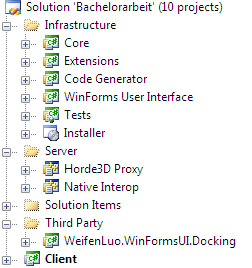
\includegraphics[scale=0.6]{images/Solution.png}
\caption{Aufbau der Visual Studio 2008 \emph{Solution}}\label{fig:solution}
\end{figure}

\subsubsection{Infrastructure}
In der Infrastruktur-Kategorie befinden sich die Projekte, die vom Client und vom Server gemeinsam benutzt werden, sowie der Code Generator und der \emph{Installer}. Alle Projekte dieser Kategorie sind in \Csharp\ geschrieben.

\begin{itemize}
	\item \textbf{Core} (DLL): Diese DLL enth�lt die Kern-Klassen des Systems. Dort befinden sich die Klassen und Interface-Definitionen f�r die Client-Server-Kommunikation, die \Horde-Klassen, die Klassen f�r das Profiling und die \Horde-Meldungen sowie \texttt{Horde3DCall} und \texttt{Horde3DDebugger}.
	
	\item \textbf{Extensions} (DLL): Dieses Projekt stellt einige n�tzliche Erweiterungen f�r das .NET Framework bereit, die vom \DevEnv\ an vielen Stellen verwendet werden.
	
	\item \textbf{Code Generator} (\emph{Executable}): Der Code Generator ist eine eigenst�ndige Anwendung zur Generierung der \Horde-\emph{Proxy}-Funktionen und -Klassen. Zur Laufzeit des Systems wird dieses Projekt nicht ben�tigt.
	
	\item \textbf{WinForms User Interface} (DLL): Diese \emph{Assembly} enth�lt die Implementierung des GUI-Frameworks unter Verwendung der Windows Forms-Klassen.
	
	\item \textbf{Tests} (DLL): Diese Bibliothek enth�lt \emph{Unit Tests} f�r das System. Derzeit gibt es allerdings nur Tests f�r das Parsen der XML-Dateien von Shader-Ressourcen.
	
	\item \textbf{Installer} (\emph{Executable}): Das Projekt erzeugt eine .msi-Datei f�r den Windows \emph{Installer}. Der \emph{Installer} kann das \DevEnv\ auf einem Computer installieren, aktualisieren und wieder l�schen. Alle Voraussetzungen -- .NET 3.5 SP1 und die Visual C++ \emph{Redistributable} f�r 32 Bit Systeme -- werden automatisch installiert.
\end{itemize}

\subsubsection{Server}
Die Server-Projekte sind .NET-\emph{Assemblies}, die in \C++/CLI geschrieben wurden. In \C++/CLI ist der Zugriff auf native Funktionen sowie die Verwendung von Zeigern einfacher und performanter als unter \Csharp. M�chte man diese \emph{Assemblies} debuggen, so ben�tigt man zun�chst eine \Horde-Anwendung, die vom \DevEnv\ gestartet wurde. Anschlie�end kann man die "`\emph{Attach Debugger}"'-Funktionalit�t von Visual Studio verwenden, um den Prozess der Anwendung zu debuggen. Zu beachten ist, dass die DLLs sowohl \emph{managed} als auch nativen Code enthalten. Der Debugger muss daher unbedingt auf "`\emph{mixed mode}"' gesetzt werden, da er ansonsten nur den nativen oder nur den \emph{managed} Teil des Codes sieht.

\begin{itemize}
	\item \textbf{Horde3D Proxy} (DLL): In dieser DLL befinden sich die \Horde-\emph{Proxy}-Funktionen sowie die globale Instanz der \texttt{Horde3DProxyHandler}-Klasse.
	
	\item \textbf{Native Interop} (DLL): Der Server f�hrt einige Aktionen durch, die sehr stark von der Win32-API abh�ngen und daher in \C++/CLI einfacher implementierbar sind. In dieser DLL befindet sich der komplette Code des \emph{Strategy Patterns} zum Anhalten der Anwendung und auch der Code zum Auslesen und Konvertieren des Inhalts eines \emph{Render Targets}.
\end{itemize}

\subsubsection{Third Party}
Zur Zeit befindet sich blo� das Projekt der Weifen Luo Winforms Docking Bibliothek in dieser Kategorie. Das \DevEnv\ verwendet zwar noch weitere Open Source Bibliotheken, diese wurden aber nicht modifiziert. In der \emph{Docking}-Bibliothek wurden hingegen ein paar kleine �nderungen vorgenommen, um das Aussehen der Shell an das von Visual Studio anzugleichen.

\subsubsection{Client}
Der Client ist das eigentliche ausf�hrbare Projekt des \DevEnvs. Vor der Kompilierung des Projekts werden die DLLs, die beim Starten des Servers in das Anwendungsverzeichnis kopiert werden m�ssen, in das \emph{Resources}-Verzeichnis des Client-Projekts kopiert. Der Compiler kompiliert dann die DLLs in die .exe-Datei als .NET-Ressource hinein. Soll der Server gestartet werden, so k�nnen die ben�tigten DLLs aus den Ressourcen ausgelesen werden. Damit entf�llt das fehleranf�llige Kopieren direkt aus dem Anwendungsverzeichnis der Shell.

Da die Verzeichnis-Struktur der \emph{Solution} nicht der Standardstruktur von Visual Studio entspricht, m�ssen zum Debuggen des Clients zwei Projekt-Einstellungen ge�ndert werden. In den Einstellungen muss im Abschnitt "`\emph{Debug}"' die "`\emph{Start Action}"' auf "`\emph{Start external program}"' gesetzt werden. Au�erdem muss der Pfad zur .exe-Datei im bin-Verzeichnis angegeben werden. Das "`\emph{Working Directory}"' muss ebenfalls auf das bin-Verzeichnis gesetzt werden.
\section{Konklusion}
F�r die Implementierung des \DevEnvs\ wurde eine Mischung aus nativem \C++, \C++/CLI und \Csharp\ verwendet. In vielen Bereichen konnten bereits vorhandene Bibliotheken gewinnbringend verwendet werden; insbesondere wurde die Umsetzung der GUI durch die Verwendung der Weifen Luo Winforms Docking Bibliothek und einiger anderer \emph{Controls} deutlich erleichtert. 

Insgesamt wurden weite Teile des Designs erfolgreich umgesetzt. Es wurde jedoch nur der Code entwickelt, der zum Erf�llen der Anforderungen erforderlich war. Gerade bei den \Horde-Klassen sind das Konzept- und auch das Designmodell jedoch detaillierter, als die Anforderungen eigentlich verlangten. An diesen Stellen wurden nur die erforderlichen Teile umgesetzt; die fehlenden Codeteile k�nnen jederzeit erg�nzt werden.

Beim Auslesen der Ressourcen-Daten fiel ein Problem mit der \Horde-API auf: Es gab keine einfache M�glichkeit, alle \Horde\ derzeit bekannten Ressourcen zu ermitteln. Jedoch wurde auf Nachfrage bei den Entwicklern eine entsprechende Funktion in \Horde\ 1.0.0 Beta 3 eingef�hrt. Die API wurde in dieser Version zus�tzlich um eine Funktion erg�nzt, die den Abschluss eines Frames markiert. Der Profiling-Mechanismus ist auf das Vorhandensein dieser Funktion angewiesen. Somit sind diese beiden Funktionen der Grund, warum das \DevEnv\ nur mit Beta 3 kompatibel ist.

Die Implementierung des GUI-Frameworks ben�tigte gegen�ber dem Designmodell einige zus�tzliche Klassen. Die neuen Klassen waren jedoch nur notwendig, um die \texttt{Shell}-, \texttt{Presenter}- und \texttt{IView}-Klassen durch Verwendung von \emph{Generics} typsicher zu machen. Das erm�glichte ein schnelleres Umsetzen der notwendigen \emph{Presenter} und \emph{Views} des \DevEnvs.

Die Erstellung des Code Generators nahm einige Zeit in Anspruch, da zun�chst die Analyse- und Design-Phasen durchlaufen werden mussten. Es zeigte sich jedoch, dass rund 4800 Zeilen Code automatisch generiert werden konnten und nicht von Hand eingetippt werden mussten. Da der Code Generator auch gut mit Updates der \Horde-API zurecht kommt, hat sich auch die detaillierte Analyse der Anforderungen und der m�glichen Probleme bei der Code Generierung gelohnt. Durch die Verwendung des GUI-Frameworks bei der Implementierung der Benutzeroberfl�che des Code Generators hielt sich der Implementierungsaufwand in Grenzen. Zudem konnten fr�h erste Erfahrungen im Umgang mit dem GUI-Framework gesammelt werden und einige Unsch�nheiten bei der Typsicherheit, der Sichtbarkeit von eigentlich internen \emph{Properties} sowie dem thread-sicheren Zugriff auf die \emph{View} eines \emph{Presenters} behoben werden.





